\section{Obecné popsání programu}
Při spuštění programu se uživateli zobrazí jednoduché a přehledné menu,  na kterém jsou 2 tlačítka: \textit{místnost1} a \textit{místnost2} viz obrázek č. 3, pokud uživatel klikne tlačítko je přesměrován do náležité místnosti. \textit{Místnost1} reprezentuje čtvercový tvar  a \textit{místnost2} reprezentuje více obdelníkový tvar místnosti. Tak je možné pozorovat různé rozdíly v tom, jak se zvuk šíří v místnostech s různými rozměry. 

    \begin{figure}[htpb]
    \centering
    \includegraphics[width=0.5\linewidth]{Obrazky/Hlavní menu.PNG}
    \caption{Hlavní menu \vspace{0.1cm}
    \newline Zdroj: vlastní}
    
    \label{fig:enter-label}
    \end{figure}
Obě místnosti jsou rozděleny na 3 části grafickou strukturou \textit{VBox}. V první části \textit{VBoxu} jsou tlačítka \textit{Stop}, \textit{Resume}, \textit{Reset}. Tlačítko \textit{Stop} simulaci zastaví, \textit{Resume} ji spustí a \textit{Reset} vymaže všechny vlny z obrazovky. Dále je na scéně zobrazen čtverec který má roli místnosti. A nakonec dole na scéně je tlačítko \textit{Hlavni Menu}, které přesměruje uživatele do hlavního menu a časovač, který slouží na časování toho jak dlouho je simulace spuštěná. Časovač  navíc slouží k indikaci, zda program běží plynule, nebo dochází k jeho zasekávání.\newpage 

\begin{figure}[htpb]
    \centering
    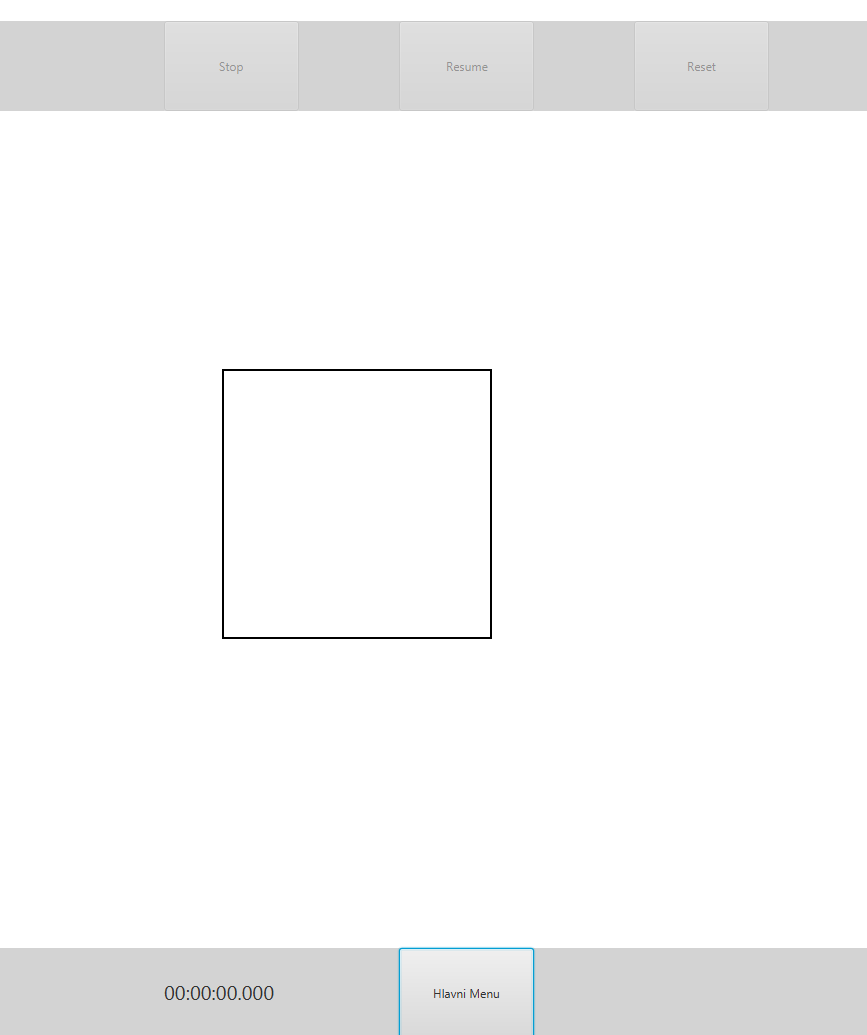
\includegraphics[width=0.7\linewidth]{Obrazky/mistnost0.png}
    \caption{Místnost 1 Zdroj: vlastní}
    \label{fig:enter-label}
\end{figure}

Pokud uživatel klikne do místnosti vytvoří se vizuální reprezentace expandující  zvukové vlny. 

\subsection{Zjednodušení}
Jelikož simulování zvukové vlny je velice náročné na grafický procesor tak bylo nutno vytvořit značně zjednodušený algoritmus, který ale bude simulovat vlnu co nejpřesněji. Mezi tato zjednodušení patří například zanedbání zmenšování amplitudy nepřímo úměrně s druhou mocninou vzdálenosti od počátku vlny. Toto rozhodnutí jsem udělal, protože by se musela počítat druhá mocnina společně s vzdáleností, což je odmocnina a dvě druhé mocniny, stokrát až tisíckrát za sekundu. Dále jsem byl nucen zanedbat počítání okamžíté výchylky v bodě pomocí vzorečku:
\[
y(t) = y_m \sin(2\pi f t + \phi)
\]

\begin{itemize}
    \item \( y_m \) - amplituda
    \item \( f \) - frekvence
    \item \( t \) - čas
    \item \( \phi \) - fáze
\end{itemize}

Rozhodl jsem se tak provést, protože počítání sinu společně s násobením desetinných čísel skoro pro každý \textit{Pixel} v místnosti je také velmi náročné. Místo toho je vlna rozdělena na několik kružnic, z nichž každá přidá či odebere pixelům okamžitou výchylku (viz kapitoly 4.11 a 4.14). To efektivně vytvoří vizuální relativně přesnou vizuální reprezentaci vlny bez toho, aniž by se program zasekával. Také bylo nutno počítat okamžitou výchylku i ostatní hodnoty důležité pro generaci vlny  pouze v integerech/ celých číslech, protože počítání v doublech/ desetinných číslech by také vyústilo v sekání programu. Jelikož je vše počítané v integerech tak ne všechny vlnové délky nebo amplitudy jsou povoleny. Proto jsem se rozhodl tyto hodnoty definovat přímo v kódu jako neměnné konstanty a to na následující hodnoty.

\begin{itemize}
    \item vlnová délka / \textit{deltaR} = 60
    \item amplituda = 100
\end{itemize}